\documentclass[../main.tex]{subfiles}

\begin{document}

\section{Edificios}

No desarrollamos mucho este tipo punto. Es necesario ver desde un punto de vista
estructural nuestros diseños. En principio, debemos ver como funcionan los \textbf{porticos}
y otros sistemas como pueden ser vigas a contraviento.

\begin{figure}[ht]
  \centering
  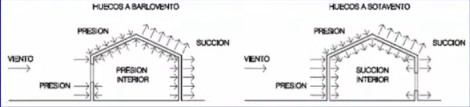
\includegraphics[width=0.8\textwidth]{../images/20210329/viento}
  \caption{Esquema de fuerzas por viento}
  \label{fig:viento}
\end{figure}

En general, estructuras de acero son muy interesante para construcciones de grandes
luces, ya que son \textit{estructuras livianas}. 


\end{document}
